% !TEX root = saveliev_physics_general_course_2.tex
%!TEX TS-program = pdflatex
%!TEX encoding = UTF-8 Unicode


\chapter{ĐIỆN TRƯỜNG TRONG ĐIỆN MÔI}\label{chap:2}

\section{Phân tử phân cực và không phân cực}\label{sec:2_1}

Điện môi (hoặc vật cách điện) được định nghĩa là chất không có khả năng dẫn điện. Vật cách điện lý tưởng không tồn tại trong tự nhiên. Với mọi chất, thậm chí là một quy mô rất nhỏ, đều dẫn điện. Nhưng chất được gọi là vật dẫn dẫn điện tốt gấp \num{e15} tới \num{e20} lần điện môi.

Nếu điện môi được đưa vào một điện trường, thì trường và bản thân điện môi chịu những thay đổi đáng kể. Để hiểu tại sao điều này xảy ra, ta phải tính đến hạt nhân và phân tử chứa điện tích hạt nhân dương và các electron tích điện âm.

Một phân tử là một hệ với tổng điện tích là không. Kích thước dài của hệ này là rất nhỏ, vào cỡ vài angstrom ( angstrom---\si{\angstrom}---là một đơn vị độ dài bằng với \SI{e-10}{\metre} rất thuận tiện trong vật lý phân tử). Chúng ta đã thành lập trong \sect{1_10} rằng trường tạo bởi hệ như vật được xác định bởi độ lớn và định hướng của moment lưỡng cực điện
\begin{equation}\label{eq:2_1}
    \vec{p} = \sum_i q_i \vec{r}_i
\end{equation}

\noindent
(tổng được thực hiện trên cả các electron và hạt nhân). Đúng vậy, các electron chuyển động trong phân tử, vì vậy moment này thay đổi liên tục. Tốc độ của các electron rất lớn, tuy nhiên, giá trị trung bình của moment \eqref{eq:2_1} được xác định trong thực tế. Vì lý do này, trong phần sau, khi đề cập tới moment lưỡng cực của một phân tử, ta đề cập đến đại lượng
\begin{equation}\label{eq:2_2}
    \vec{p} = \sum_i q_i \average{\vec{r}_i}
\end{equation}

\noindent
(đối với hạt nhân, $\vec{r}_i$ được lấy đơn giản là $\average{\vec{r}_i}$ trong tổng này). Nói cách khác, ta sẽ xem các electron là đứng yên so với hạt nhân tại các điểm nhất định thu được bằng cách lấy trung bình vị trí của electron theo thời gian.

Hành vi của phân tử trong điện trường ngoài cũng được xác định bởi moment lưỡng cực của nó. Ta có thể xác nhận điều này bằng cách tính thế năng của một phân tử trong điện trường ngoài. Chọn gốc tọa độ bên trong phân tử và lợi dụng độ nhỏ của $\average{\vec{r}_i}$, ta viết điện thế tại điểm của điện tích thứ $i$ có dạng
\begin{equation*}
    \varphi_i = \varphi + \gradop{\varphi} \ccdot \average{\vec{r}_i}
\end{equation*}

\noindent
với $\varphi$ là điện thế tại gốc tọa độ [xem \eqn{1_69}]. Do đó,
\begin{equation*}
    \ab{W}{p} = \sum_i q_i \varphi_i = \sum_i q_i \parenthesis{\varphi + \gradop{\varphi} \ccdot \average{\vec{r}_i}} = \varphi \sum_i q_i + \gradop{\varphi} \sum_i q_i \average{\vec{r}_i}.
\end{equation*}

\noindent
Tính đến $\sum_i q_i=0$ và thay $-\vec{E}$ cho $\gradop{\varphi}$, ta được
\begin{equation*}
    \ab{W}{p} = -\vec{E} \sum_i q_i \average{\vec{r}_i} = -\vecdot{p}{E} = -p E \cos\alpha.
\end{equation*}

\noindent
Vi phân biểu thức này theo $\alpha$, ta được \eqn{1_57} cho moment quay; vi phân theo $x$, ta được lực \eqref{eq:1_62}.

Do đó, một phân tử tương đương với một lưỡng cực cả về trường nó thiết lập và lực nó chịu tác dụng trong trường ngoài. Điện tích dương của lưỡng cực này bằng với tổng điện tích của hạt nhân và đặt tại ``tâm tỷ cự'' của các điện tích dương; điện tích âm bằng với tổng điện tích của các electron và đặt tại ``tâm tỷ cự'' của các điện tích âm.

Trong phân tử đối xứng (như \ce{H2},\ce{O2}, \ce{N2}), tâm tỷ cự của các điện tích âm và dương trùng nhau khi không có mặt điện trường ngoài. Những phân tử như vậy không có moment lưỡng cực riêng và được gọi là \textbf{không phân cực}. Trong phân tử bất đối xứng (như là \ce{CO}, \ce{NH}, \ce{HCl}), tâm tỷ cự của các điện tích trái dấu không trùng nhau. Trong trường hợp này, phân tử có moment lưỡng cực riêng và gọi là \textbf{phân cực}.

Dưới tác dụng của điện trường ngoài, các điện tích trong phân tử không phân cực dịch chuyển tương đối so với nhau, điện tích dương theo hướng của trường, điện tích âm theo hướng ngược lại. Kết quả là, phân tử nhận được một moment lưỡng cực mà độ lớn của nó, như được chỉ ra bởi thực nghiệm, tỷ lệ với cường độ trường. Trong điều kiện chuẩn hóa, hằng số tỷ lệ được viết ở dạng $\varepsilon_0\beta$, với $\varepsilon_0$ là hằng số điện, và $\beta$ là một đại lượng được gọi là \textbf{độ phân cực của phân tử}. Vì hướng của $\vec{p}$ và $\vec{E}$ trùng nhau, ta có thể viết
\begin{equation}\label{eq:2_3}
    \vec{p} = \beta \varepsilon_0 \vec{E}.
\end{equation}

\noindent
Moment lưỡng cực có thứ nguyên [$q$]L. Theo \eqn{1_15}, thứ nguyên của $\varepsilon_0\vec{E}$ là [$q$]L$^{-2}$. Do đó, độ phân cực của phân tử $\beta$ có thứ nguyên L$^3$.

Quá trình phân cực của một phân tử không phân cực diễn ra như thể các điện tích dương và âm của phân tử được liên kết với nhau bằng lực đàn hồi. Một phân tử không phân cực, do đó gọi là, hành xử trong trường ngoài như một lưỡng cực đàn hồi.

Tác động của trường ngoài lên phân tử phân cực chủ yếu có xu hướng quay phân tử sao cho moment lưỡng cực được xếp theo hướng của trường. Trường ngoài hầu như không ảnh hưởng đến độ lớn của moment lưỡng cực. Kết quả là, phân tử phân cực hành xử trong trường ngoài như một lưỡng cực cứng.

\section{Phân cực điện môi}\label{sec:2_2}

Khi không có điện trường ngoài, moment lưỡng cực phân tử của điện môi thường hoặc là bằng không (phân tử không phân cực) hoặc là phân bố trong không gian với hướng hỗn loạn (phân tử phân cực). Trong cả hai trường hợp, moment lưỡng cực tổng cộng của điện môi bằng không\footnote{Trong \sect{2_9}, ta sẽ làm quen với những chất có thể có moment lưỡng cực khi không có trường ngoài.}.
    
Điện môi trở nên phân cực dưới tác động của trường ngoài. Điều này có nghĩa là moment lưỡng cực tổng hợp của điện môi khác không. Hoàn toàn tự nhiên khi lấy moment lưỡng cực trên đơn vị thể tích như đại lượng đặc trưng cho độ phân cực. Nếu trường hoặc điện môi (hoặc cả hai) không đồng chất, độ phân cực tại các điểm khác nhau của điện môi sẽ khác nhau. Để đặc trưng cho độ phân cực tại một điểm, ta phải tách ra một thể tích nhỏ vô cùng $\Delta{V}$ chứa điểm này, tìm tổng $\sum_{\Delta{V}}\vec{p}$ của những phân tử giới hạn trong thể tích này, và lấy tỷ lệ
\begin{equation}\label{eq:2_4}
    \vec{P} = \frac{\displaystyle\sum_{\Delta{V}}\vec{p}}{\Delta{V}}.
\end{equation}

\noindent
Đại lượng vector $\vec{P}$ định nghĩa bởi \eqn{2_4} được gọi là \textbf{độ phân cực điện môi}.

Moment lưỡng cực $\vec{p}$ có thứ nguyên là [$q$]L. Do đó, thứ nguyên của $\vec{P}$ là [$q$]L$^{-2}$, tức là, giống với thứ nguyên của $\varepsilon_0\vec{E}$ [xem \eqn{1_15}].

Độ phân cực của bất kỳ loại điện môi đẳng hướng nào được liên kết với cường độ trường tại cùng một điểm bởi mối liên hệ đơn giản
\begin{equation}\label{eq:2_5}
    \vec{P} = \chi \varepsilon_0 \vec{E}
\end{equation}

\noindent
với $\chi$ là một đại lượng độc lập với $\vec{E}$ gọi là \textbf{độ cảm điện của điện môi}\footnote{trong điện môi bất đẳng hướng, hướng của $\vec{P}$ và $\vec{E}$, nói chung, không trùng nhau. Trong trường hợp này, mối liên hệ giữa $\vec{P}$ và $\vec{E}$ được mô tả bởi phương trình
\begin{align*}
    P_x &= \varepsilon\parenthesis{\chi_{xx}E_x + \chi_{xy}E_y+\chi_{xz}E_z},\\
    P_y &= \varepsilon\parenthesis{\chi_{yx}E_x + \chi_{yy}E_y+\chi_{yz}E_z},\\
    P_z &= \varepsilon\parenthesis{\chi_{zx}E_x + \chi_{zy}E_y+\chi_{zz}E_z}.
\end{align*}

\noindent
Sự kết hợp của chín đại lượng $\chi_{ij}$ tạo thành một tensor đối xứng bậc hai gọi là \textbf{tensor của độ cảm điện điện môi} [so sánh với Eqs. (5.30)
của Vol. I). Tensor này đặc trưng cho những tính chất điện của điện môi dị hướng.}. Ở trên ta đã đề cập về thứ nguyên của $\vec{P}$ và $\varepsilon_0\vec{E}$ là giống nhau. Do đó, $\chi$ là một đại lượng không thứ nguyên.

Trong hệ đơn vị Gauss, \eqn{2_5} có dạng
\begin{equation}\label{eq:2_6}
    \vec{P} = \chi \vec{E}.
\end{equation}

Với điện môi tạo thành từ những phân tử không phân cực, \eqn{2_5} nhận được từ những xem xét đơn giản sau. Thể tích $\Delta{V}$ chứa $n\Delta{V}$ phân tử, với $n$ là số phân tử trên đơn vị thể tích. Mỗi moment $\vec{p}$ được xác định trong trường hợp này bởi \eqn{2_3}. Do đó,
\begin{equation*}
    \sum{\Delta{V}} \vec{p} = n \Delta{V} \beta \varepsilon_0 \vec{E}.
\end{equation*}

\noindent
Chia biểu thức này cho $\Delta{V}$, ta được độ phân cực $\vec{P}=n\beta\varepsilon_0\vec{E}$. Cuối cùng, ký hiệu $\chi=n\beta$, ta được \eqn{2_5}.

Với điện môi tạo thành từ những phân tử phân cực, tác động định hướng của trường ngoài bị chống lại bởi chuyển động nhiệt của phân tử có xu hướng phân tán moment lưỡng cực của nó theo mọi hướng. Kết quả là, một hướng ưu tiên của moment lưỡng cực được thiết lập theo hướng của trường. Các tính toán thống kê liên quan, phù hợp với số liệu thực nghiệm, chỉ ra rằng độ phân cực tỷ lệ thuận với cường độ trường, tức là, dẫn đến \eqn{2_5}. Độ cảm điện của những điện môi như vậy tỷ lệ nghịch với nhiệt độ tuyệt đối.

Trong tinh thể ion, các phân tử riêng lẻ mất đi tính độc lập của chúng. Toàn bộ tinh thể, như nó đã từng, là một phân tử lớn duy nhất. Mạng tinh thể của một tinh thể ion có thể được xem như hai mạng lồng vào nhau, một trong số đó được tạo thành bởi ion dương, và cái còn lại bởi ion âm. Khi một trường ngoài tác động lên các ion tinh thể, hai mạng di chuyển tương đối với nhau, dẫn đến sự phân cực của điện môi. Sự phân cực trong trường hợp này cũng kết hợp với cường độ trường bởi \eqn{2_5}. Ta phải chú ý rằng liên hệ tuyến tính giữa $\vec{E}$ và $\vec{P}$ mô tả bởi \eqn{2_5} chỉ được áp dụng với trường không quá mạnh [chú ý tương tự cho \eqn{2_3}].

\section{Trường bên trong điện môi}\label{sec:2_3}

Các điện tích trong các phân tử điện môi được gọi là \textbf{điện tích liên kết}. Tác động của một trường chỉ có thể làm điện tích liên kết dịch chuyển nhỏ khỏi vị trí cân bằng của chúng; không thể thoát khỏi phân tử chứa nó.

Theo ví dụ của L. Landau và E. Lifshitz\footnote{Xem L. D. Landau and E. M. Lifshitz. Elektrodinamika sploshnykh sred (Electrodynamics of Continuous Media). Moscow, Gostekhizdat (1957), p. 57.}, ta sẽ gọi các điện tích mà, mặc dù nằm trong giới hạn của điện môi, nhưng không nằm trong các phân tử, và cả các điện tích nằm bên ngoài điện môi, là các điện tích ngoài\footnote{Thông thường ta gọi những điện tích này \textbf{tự do}. Tuy nhiên cái tên này không chính xác bởi vì trong một số trường hợp điện tích ngoài không tự do.}.

Trường trong điện môi là chồng chất của trường $\ab{\vec{E}}{extr}$ tạo bởi các điện tích ngoài, và trường $\ab{\vec{E}}{bound}$ của các điện tích liên kết. Trường tổng hợp được gọi là \textbf{vi mô} (hoặc \textbf{đúng}):
\begin{equation}\label{eq:2_7}
    \ab{\vec{E}}{micro} = \ab{\vec{E}}{extr} + \ab{\vec{E}}{bound}.
\end{equation}

Trường vi mô thay đổi mạnh trong giới hạn khoảng cách liên phân tử. Do chuyển động của các điện tích liên kết, trường $\ab{\vec{E}}{micro}$ cũng thay đổi theo thời gian. Những thay đổi này không bị phát hiện trong thang vĩ mô. Do đó, một trường được đặc trưng bởi đại lượng \eqref{eq:2_7} trung bình trên một thể tích vô cùng nhỏ, túc là,
\begin{equation*}
    \vec{E} = \average{\ab{\vec{E}}{micro}} = \average{\ab{\vec{E}}{extr}} + \average{\ab{\vec{E}}{bound}}.
\end{equation*}

Sau đây, ta sẽ ký hiệu trường trung bình của các điện tích ngoài là $\vec{E}_0$, và trường trung bình của các điện tích liên kết là $\vec{E}'$. Theo đó, ta định nghĩa trường vĩ mô là đại lượng
\begin{equation}\label{eq:2_8}
    \vec{E} = \vec{E}_0 + \vec{E}'.
\end{equation}

Độ phân cực $\vec{P}$ là một đại lượng vĩ mô. Do đó, $\vec{E}$ trong \eqn{2_5} nên được hiểu là trường xác định bởi \eqn{2_8}.

Khi không có điện môi (tức là, trong chân không), trường vĩ mô là
\begin{equation*}
    \vec{E} = \vec{E}_0 = \average{\ab{\vec{E}}{extr}}.
\end{equation*}

\noindent
Nó chính xác là đại lượng được hiểu là $\vec{E}$ trong \eqn{1_117}.

Nếu các điện tích ngoài tĩnh, trường xác định bởi \eqn{2_8} có cùng tính chất như một điện trường tĩnh trong chân không. Đặc biệt, nó có thể được mô tả bằng điện thế $\varphi$ liên quan tới cường độ trường \eqref{eq:2_8} bởi Eqs. \eqref{eq:1_41} và \eqref{eq:1_45}.

\section{Điện tích liên kết mặt và khối}\label{sec:2_4}

Khi điện môi không phân cực, mật độ điện khối $\rho'$ và mật độ điện mặt $\sigma'$ của các điện tích liên kết bằng không. Sự phân cực gây ra mật độ điện mặt, và trong vài trường hợp mật độ điện khối của điện tích liên kết cũng trở nên khác không.

Hình \ref{fig:2_1} minh họa sơ đồ điện môi phân cực của phân tử không phân cực (a) và phân cực (b). Quan sát hình vẽ cho thấy sự phân cực xảy ra khi xuất hiện các điện tích liên kết dư thừa cùng dấu trong lớp mỏng bề mặt của điện môi. Nếu thành phần pháp tuyến của cường độ trường $\vec{E}$ đối với tiết diện đã cho của bề mặt khác không, thì dưới tác động của trường, điện tích của một dấu sẽ di chuyển vào bên trong và dấu kia sẽ xuất hiện ở bề mặt.

\begin{figure}[!htb]
	\begin{minipage}[t]{0.64\linewidth}
		\begin{center}
			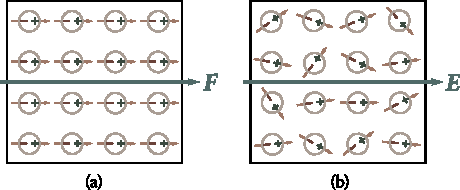
\includegraphics[scale=1]{figures/ch_02/fig_2_1.pdf}
			\caption[]{}
			\label{fig:2_1}
		\end{center}
	\end{minipage}
	\hfill{}%space{-0.05cm}
	\begin{minipage}[t]{0.34\linewidth}
		\begin{center}
			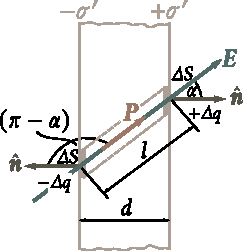
\includegraphics[scale=1]{figures/ch_02/fig_2_2.pdf}
			\caption[]{}
			\label{fig:2_2}
		\end{center}
	\end{minipage}
\vspace{-0.4cm}
\end{figure}

Có một liên hệ đơn giản giữa độ phân cực $\vec{P}$ và mật độ điện tích liên kết mặt $\sigma'$. Để tìm nó, ta  xét một bản mặt song song vô hạn của điện môi đồng chất đặt trong một điện trường đồng nhất (\fig{2_2}). Ta hãy tách ra một thể tích nguyên tố trong bản ở dạng một hình trụ rất mỏng có đường sinh song song với $\vec{E}$ trong điện môi, và có diện tích đáy $\Delta{S}$ trùng với bề mặt bản. Độ lớn của thể tích này là
\begin{equation*}
    \Delta{V} = l \Delta{S} \cos\alpha
\end{equation*}

\noindent
Với $l$ là khoảng cách giữa các đáy của hình trụ và $\alpha$ là góc giữa vector $\vec{E}$ và một ngoại hướng pháp tuyến với bề mặt tích điện dương của điện môi.

Thể tích $\Delta{V}$ có moment lưỡng cực điện với độ lớn
\begin{equation*}
    P\Delta{V} = Pl\Delta{S}\cos\alpha
\end{equation*}

\noindent
($P$ là độ lớn của độ phân cực).

Theo quan điểm vĩ mô, thể tích có thể được xem như tương đương với một lưỡng cực tạo bởi $+\sigma'\Delta{S}$ và $-\sigma'\Delta{S}$ với khoảng cách $l$. Do đó, moment điện của nó có thể được viết ở dạng $\sigma'\Delta{S}l$. Đồng nhất hai biểu thức cho moment điện, ta có
\begin{equation*}
    Pl\Delta{S}\cos\alpha = \sigma'\Delta{S}l.
\end{equation*}

\noindent
Do đó, ta nhận được mối qua hệ cần thiết giữa $\sigma'$ và $\vec{P}$:
\begin{equation}\label{eq:2_9}
    \sigma' = P \cos\alpha = \ab{P}{n}
\end{equation}

\noindent
với $\ab{P}{n}$ là hình chiếu của độ phân cực lên một ngoại hướng pháp tuyến của bề mặt liên quan. Ở bề mặt bên phải trong \fig{2_2}, ta có $\ab{P}{n}>0$, theo đó, $\sigma'$ cho nó là dương; ở bề mặt bên trái $\ab{P}{n}<0$, theo đó, $\sigma'$ của nó là âm.

Biểu diễn $\vec{P}$ qua $\chi$ và $\vec{E}$ bằng \eqn{2_5}, ta được công thức
\begin{equation}\label{eq:2_10}
    \sigma' = \chi \varepsilon_0 \ab{E}{n}
\end{equation}

\noindent
với $\ab{E}{n}$ là thành phần pháp tuyến của cường độ trường bên trong điện môi. Theo \eqn{2_10}, tại nơi đường sức trường đi ra khỏi điện môi ($\ab{E}{n}>0$), điện tích liên kết dương xuất hiện ở bề mặt, trong khi tại nơi đường sức trường đi vào  điện môi ($\ab{E}{n}<0$), điện tích mặt âm xuất hiện.

Phương trình \eqref{eq:2_9} và \eqref{eq:2_10} vẫn đúng trong trường hợp tổng quát nhất khi một điện môi không đồng chất hình dạng bất kỳ đặt trong một điện trường không đồng nhất. Với $\ab{P}{n}$ và $\ab{E}{n}$ trong trường hợp này, ta phải hiểu thành phần pháp tuyến của vector liên quan được lấy gần trực tiếp với bề mặt nguyên tố mà $\sigma'$ được xác định.

Bây giờ ta hãy tìm mật độ khối của điện tích liên kết bên trong điện môi không đồng chất. Xét một diện tích ảo nhỏ $\Delta{S}$ (\fig{2_3}) trong điện môi đẳng hướng không đồng chất với phân tử không phân cực.
Cho rằng một đơn vị thể tích điện môi có $n$ hạt giống hệt nhau với điện tích $+e$ và $n$ hạt giống hệt nhau với điện tích $-e$. Ở gần diện tích $\Delta{S}$, điện trường và điện môi có thể được xem là đồng nhất.
Do đó, khi trường xuất hiện, mọi điện tích dương gần $\Delta{S}$ sẽ dịch chuyển một khoảng cách bằng nhau $l_1$ theo hướng của $\vec{E}$, và mọi điện tích âm sẽ dịch chuyển theo hướng ngược lại cùng một đoạn $l_2$ (xem \fig{2_3}).
Một số điện tích nhất định cùng dấu (dương nếu $\alpha<\pi/2$ và âm nếu $\alpha>\pi/2$) sẽ đi qua diện tích $\Delta{S}$ theo hướng của một pháp tuyến với nó, và một số điện tích nhất định trái dấu (âm nếu $\alpha<\pi/2$ và dương nếu $\alpha<\pi/2$) theo hướng ngược với $\hatvec{n}$.
Diện tích $\Delta{S}$ sẽ bị cắt bởi tất cả tất cả điện tích $+e$ nằm cách nó một khoảng không quá $l_1\cos\alpha$ trước khi trường được bật, tức là, bởi tất cả $+e$ trong hình trụ xiên có thể tích $l_1\Delta{S}\cos\alpha$. Lượng điện tích này là $nl_1\Delta{S}\cos\alpha$, trong khi điện tích chúng mang theo hướng của pháp tuyến tới diện tích là $enl_1\Delta{S}\cos\alpha$ (khi $\alpha>\pi/2$, điện tích được mang theo hướng của pháp tuyến do sự dịch chuyển của điện tích $+e$ là âm).
Tương tự, diện tích $\Delta{S}$ sẽ bị cắt bởi tất cả điện tích $-e$ trong thể tích $l_2\Delta{S}\cos\alpha$. Những điện tích này sẽ mang điện tích $enl_2\Delta{S}\cos\alpha$ theo hướng pháp tuyến của diện tích (từ \fig{2_3} chỉ ra rằng khi $\alpha<\pi/2$, điện tích $-e$ sẽ mang lượng điện tích $-enl_2\Delta{S}\cos\alpha$ qua $\Delta{S}$ theo hướng ngược với $\hatvec{n}$, tương đương với việc mang điện tích $enl_2\Delta{S}\cos\alpha$ theo hướng của $\hatvec{n}$).

\begin{figure}[!htb]
	\begin{center}
		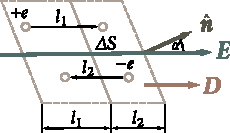
\includegraphics[scale=1.1]{figures/ch_02/fig_2_3.pdf}
		\caption[]{}
		\label{fig:2_3}
	\end{center}
	\vspace{-0.8cm}
\end{figure}

Do đó, khi trường được bật, điện tích
\begin{equation*}
    \Delta{q}' = enl_1\Delta{S}\cos\alpha + enl_2\Delta{S}\cos\alpha = en (l_1+l_2) \Delta{S} \cos\alpha
\end{equation*}

\noindent
được mang qua diện tích $\Delta{S}$ theo hướng pháp tuyến của nó. Tổng $l_1+l_2$ là khoảng cách $l$ mà điện tích liên kết dịch chuyển về phía nhau trong điện môi.Như là kết quả của của sự dịch chuyển này, mỗi cặp điện tích nhận được moment lưỡng cực $p=el=e(l_1+l_2)$. Số cặp trong trong một đơn vị thể tích là $n$. Kết quả là, tích $e(l_1+l_2)n=eln=p$ cho ta độ lớn của độ phân cực $P$. Từ đó, điện tích đi qua diện tích $\Delta{S}$ theo hướng pháp tuyến khi trường được bật là [xem \eqn{2_9}]
\begin{equation*}
    \Delta{q}' = P \Delta{S} \cos\alpha.
\end{equation*}

Vì điện môi đẳng hướng, hướng của vector $\vec{E}$ và $\vec{P}$ trùng nhau (xem \fig{2_3}). Kết quả là, $\alpha$ là góc giữa vector $\vec{P}$ và $\hatvec{n}$, và trong liên hệ này ta có thể viết
\begin{equation*}
    \Delta{q}' = (\vec{P} \ccdot \hatvec{n})\, \Delta{S}.
\end{equation*}

\noindent
Chuyển từ $\Delta$ sang vi phân, ta có
\begin{equation*}
    \deriv{q} = (\vec{P} \ccdot \hatvec{n})\, \deriv{S} = \vec{P} \ccdot \deriv{\vec{S}}.
\end{equation*}

Ta đã tìm được điện tích liên kết $\deriv{q'}$ mà đi qua diện tích nguyên tố $\deriv{S}$ theo hướng pháp tuyển khi trường được bật; $\vec{P}$ là độ phân cực thiết lập dưới tác dụng của điện trường tại vị trí diện tích $\deriv{S}$.

Tưởng tượng một mặt đóng $S$ bên trong điện môi. Khi trường được bật, một điện tích liên kết $q'$ sẽ cắt bề mặt này và đi ra từ nó. Điện tích này là
\begin{equation*}
    \ab{q'}{em} = \oint_S \deriv{q'} = \oint_S \vec{P} \ccdot \deriv{\vec{S}}
\end{equation*}

\noindent
(ta đã đồng ý lấy ngoại hướng pháp tuyến cho diện tích $\deriv{S}$ của mặt kín). Kết quả là, một điện tích liên kết dư sẽ xuất hiện trong thể tích giới hạn bởi bề mặt $S$. Giá trị của nó là
\begin{equation}\label{eq:2_11}
    \ab{q'}{sur} = - \ab{q'}{em} = - \oint_S \vec{P} \ccdot \deriv{\vec{S}} = - \ab{\Phi}{P}
\end{equation}

\noindent
($\ab{\Phi}{P}$ là thông lượng của vector $\vec{P}$ qua mặt $S$).

Đưa vào mật độ điện tích liên kết khối $\rho'$, ta có thể viết
\begin{equation*}
    \ab{q'}{sur} = \int_V \rho'\, \deriv{V}
\end{equation*}

\noindent
(tích phân được lấy trên toàn bộ thể tích giới hạn bởi bề mặt $S$). Chúng ta do đó có được công thức
\begin{equation*}
    \int_V \rho'\, \deriv{V} = - \oint_S \vec{P} \ccdot \deriv{\vec{S}}.
\end{equation*}

\noindent
Biến đổi tích phân mặt theo định lý Ostrogradsky-Gauss [xem \eqn{1_108}). Kết quả là
\begin{equation*}
    \int_V \rho'\, \deriv{V} = - \int_V \divop{\vec{P}}\, \deriv{V}.
\end{equation*}

\noindent
Phương trình này phải được tuân thủ cho bất kì thể tích được chọn tùy ý $V$. Điều này chỉ có thể xảy ra nếu phương trình sau được tuân thủ tại mọi điểm của điện môi:
\begin{equation}\label{eq:2_12}
    \rho' = - \divop{\vec{P}}.
\end{equation}

\noindent
Kết quả là, mật độ điện tích liên kết bằng với divergence của độ phân cực $\vec{P}$ lấy trái dấu.

Ta nhận được \eqn{2_12} khi xét điện môi với phân tử không phân cực. Phương trình này vẫn đúng cho điện môi với phân tử phân cực.

\begin{figure}[!htb]
	\begin{center}
		
\includegraphics[scale=1]{figures/ch_02/fig_2_4.pdf}
		\caption[]{}
		\label{fig:2_4}
	\end{center}
	\vspace{-0.8cm}
\end{figure}

Phương trình \eqref{eq:2_12} có thể giải thích bằng sơ đồ. Các điểm với $\divop{\vec{P}}$ dương là nguồn của trường vector $\vec{P}$, và các đường sức từ $\vec{P}$ phân kì từ chúng (\fig{2_4}). Các điểm với $\divop{\vec{P}}$ âm là phần chìm của trường vector $\vec{P}$, và các đường sức của $\vec{P}$ hội tụ tại chúng.
Trong sự phân cực điện môi, các điện tích liên kết dương dịch chuyển theo hướng của vector $\vec{P}$, tức là, theo hướng của các đường $\vec{P}$; Các điện tích liên kết âm dịch chuyển theo hướng ngược lại (trong hình các điện tích liên kết thuộc về các phân tử riêng biệt được bao quanh bởi hình bầu dục). Kết quả là, sự dư thừa các điện tích liên kết âm được tạo thành tại những điểm có $\divop{\vec{P}}$ dương, và sự dư thừa các điện tích liên kết dương tại nơi có $\divop{\vec{P}}$ âm.
 Điện tích liên kết chỉ khác điện tích ngoài ở chỗ chúng không thể rời khỏi giới hạn phân tử của chúng. Nếu không thì, chúng có cùng đặc tính với toàn bộ điện tích khác. Đặc biệt, chúng là nguồn của một điện trường. Do đó, khi mật độ điện tích liên kết $\rho'$ khác không, \eqn{1_117} phải được viết ở dạng
\begin{equation}\label{eq:2_13}
    \divop{\vec{E}} = \frac{1}{\varepsilon_0} \parenthesis{\rho + \rho'}.
\end{equation}

\noindent
Ở đây $\rho$ là mật độ điện tích ngoài.

Đưa \eqn{2_5} for $\vec{P}$ vào \eqn{2_12} và sử dụng \eqn{1_103}. Kết quả là
\begin{equation*}
    \rho' = - \divop{(\chi\varepsilon_0\vec{E})} = - \varepsilon_0 \divop{(\chi\vec{E})} = - \varepsilon_0 [\vec{E}\ccdot\gradop{\chi} + \chi \divop{\vec{E}}].
\end{equation*}

\noindent
Thay thể $\divop{\vec{E}}$ bằng giá trị của nó từ \eqn{2_13}, ta nhận được phương trình
\begin{equation*}
    \rho' = - \varepsilon_0 (\vec{E}\ccdot\gradop{\chi}) - \chi\rho - \chi\rho'.
\end{equation*}

\noindent
Vì thế,
\begin{equation}\label{eq:2_14}
    \rho' = - \parenthesis{\frac{1}{1+\chi}} [\varepsilon_0 (\vec{E}\ccdot\gradop{\chi}) + \chi\rho].
\end{equation}

Ta có thể thấy từ \eqn{2_14} rằng mật độ điện tích liên kết khối có thể khác không trong hai trường hợp: (1) nếu điện môi không đồng nhất ($\gradop{\chi}\neq 0$), và (2) nếu tại một khu vực cho trước trong điện môi. mật độ điện tích ngoài khác không ($\rho\neq 0$).

Khi không có điện tích ngoài trong điện môi, mật độ điện tích liên kết khối là
\begin{equation}\label{eq:2_15}
    \rho' = - \parenthesis{\frac{\varepsilon_0}{1+\chi}} (\vec{E}\ccdot\gradop{\chi}).
\end{equation}

\section{Vector điện dịch}\label{sec:2_5}

Ta chú ý ở phần trước rằng không chỉ có điện tích ngoài, mà điện tích liên kết cũng là nguồn của trường. Theo,
\begin{equation}\label{eq:2_16}
    \divop{\vec{E}} = \frac{1}{\varepsilon_0} \parenthesis{\rho + \rho'}
\end{equation}

\noindent
[xem \eqn{2_13}].

Phương trình \eqref{eq:2_16} hầu như không dùng để tìm vector $\vec{E}$ bởi vì nó thể hiện đặc tính của đại lượng chưa biết $\vec{E}$ thông qua điện tích liên kết, cái mà được xác định bởi đại lượng $\vec{E}$ chưa biết [xem phương trình \eqref{eq:2_10} và \eqref{eq:2_14}].

Tính toán trường thường được đơn giản hóa khi ta đưa vào một đại lượng phụ mà nguồn của nó chỉ là các điện tích ngoài $\rho$. Để thiết lập đại lượng này trông như thế nào, ta đưa vào \eqn{2_12} của $\rho'$ vào \eqn{2_16}:
\begin{equation*}
    \divop{\vec{E}} = \frac{1}{\varepsilon_0} (\rho - \divop{\vec{P}})
\end{equation*}

\noindent
Theo đó
\begin{equation}\label{eq:2_17}
    \divop{(\varepsilon_0\vec{E} + \vec{P})} = \rho
\end{equation}

\noindent
(Ta đặt $\varepsilon_0$ trong ký hiệu del). Biểu thức trong dấu ngoặc đơn trong \eqn{2_17} là đại lượng cần tìm. Nó được ký hiệu bởi $\vec{D}$ và được gọi là vector điện dịch (hoặc cảm ứng điện).

Do đó, vector \textbf{điện dịch} là một đại lượng xác định bởi liên hệ
\begin{equation}\label{eq:2_18}
    \vec{D} = \varepsilon_0\vec{E} + \vec{P}.
\end{equation}

\noindent
Thay \eqn{2_5} cho $\vec{P}$, ta có
\begin{equation}\label{eq:2_19}
    \vec{D} = \varepsilon_0\vec{E} + \chi\varepsilon_0\vec{E} = \varepsilon_0 (1+\chi) \vec{E}.
\end{equation}

Đại lượng vô hướng
\begin{equation}\label{eq:2_20}
    \varepsilon = 1 + \chi
\end{equation}

\noindent
được gọi là \textbf{hằng số điện môi tương đối} hoặc đơn giản là \textbf{hằng số điện môi} của môi trường\footnote{Cái gọi là hằng số điện môi tuyệt đối của môi trường $\ab{\varepsilon}{a}=\varepsilon_0\varepsilon$ được giới thiệu trong kỹ thuật điện. Đại lượng này bị thiếu đi ý nghĩa vật lý, tuy nhiên, ta sẽ không dùng nó.}. Do đó, \eqn{2_19} có thể được viết ở dạng
\begin{equation}\label{eq:2_21}
    \vec{D} = \varepsilon_0 \varepsilon \vec{E}.
\end{equation}

\noindent
Theo \eqn{2_21}, vector $\vec{D}$ tỷ lệ với vector $\vec{E}$. Nhắc lại cho người đọc rằng chúng ta đang giải quyết với điện môi đẳng hướng. Trong điện môi không đẳng hướng, vector $\vec{E}$ và $\vec{D}$, nói chung, là không thẳng hàng.

Phù hợp với \eqn{1_15} và \eqn{2_21}, vector điện dịch của trường của một điện tích điểm trong chân không là
\begin{equation}\label{eq:2_22}
    \vec{D} = \frac{1}{4\pi} \frac{q}{r^2} \vecuni{r}.
\end{equation}

Đơn vị của độ điện dịch là coulomb trên mét bình phương (\si{\coulomb\per\metre\squared}).

Phương trình \eqref{eq:2_17} có thể được viết như
\begin{equation}\label{eq:2_23}
    \divop{\vec{D}} = \rho.
\end{equation}

\noindent
Tích phân phương trình này trên một thể tích bất kỳ $V$ dẫn đến
\begin{equation*}
    \int_V \divop{\vec{D}}\, \deriv{V} = \int_V \rho\, \deriv{V}.
\end{equation*}

\noindent
Ta hãy biến đổi vế trái theo định lý Ostrogradsky-Gauss [xem \eqn{1_108}]:
\begin{equation}\label{eq:2_24}
    \oint_S \vec{D} \ccdot \deriv{\vec{S}} = \int_V \rho\, \deriv{V}.
\end{equation}

\noindent
Đại lượng bên vế trái là $\Phi_D$---thông lượng của vector $\vec{D}$ qua mặt kín $S$, trong khi đó ở vế phải là tổng điện tích ngoài $\sum_iq_i$ giới hạn bởi bề mặt này. Do đó, \eqn{2_24} có thể được viết ở dạng
\begin{equation}\label{eq:2_25}
    \Phi_D = \sum_i q_i.
\end{equation}

\noindent
Phương trình \eqref{eq:2_24} và \eqref{eq:2_25} thể hiện định luật Gauss cho vector $\vec{D}$: \textit{thông lượng điện dịch qua một mặt kín bằng tổng đại số của điện tích ngoài giới hạn trong mặt này}.

Trong chân không, $\vec{P}=0$, vì vậy đại lượng $\vec{D}$ xác định bởi \eqn{2_18} chuyển thành $\varepsilon_0\vec{E}$, phương trình \eqref{eq:2_24} và \eqref{eq:2_25} chuyển thành phương trình \eqref{eq:1_114} và \eqref{eq:1_116}.

Đơn vị của thông lượng vector điện dịch là coulomb. Xem \eqn{2_25}, một điện tích \SI{1}{\coulomb} tạo ra thông lượng điện dịch \SI{1}{\coulomb} qua bề mặt bao quanh nó.

Trường của vector $\vec{D}$ có thể minh họa bằng các đường điện dịch (ta sẽ gọi chúng là các đường dịch cho ngắn gọn). Hướng và mật độ của chúng được xác định theo cách giống hệt như các đường của vector $\vec{E}$ (xem \sect{1_5}). Các đường của vector $\vec{E}$ có thể bắt đầu và kết thúc tại cả điện tích ngoài và liên kết. Nguồn của trường vector $\vec{D}$ chỉ là điện tích ngoài. Do đó, các đường dịch chỉ có thể bắt đầu và kết thúc tại điện tích ngoài. Những đường này đi qua mà không bị ngắt quãng tại các điểm có điện tích liên kết.

Cảm ứng điện\footnote{Thuật ngữ ``điện dịch'' không áp dụng cho đại lượng \eqref{eq:2_27}.} trong hệ Gauss được xác định bởi biểu thức
\begin{equation}\label{eq:2_26}
    \vec{D} = \vec{E} + 4\pi\vec{P}.
\end{equation}

\noindent
Thay $\vec{P}$ trong phương trình này bằng giá trị của nó trong \eqn{2_6}, ta có
\begin{equation}\label{eq:2_27}
    \vec{D} = (1 + 4\pi\chi) \vec{E}.
\end{equation}

Đại lượng
\begin{equation}\label{eq:2_28}
    \varepsilon = 1 + 4\pi\chi.
\end{equation}

\noindent
được gọi là \textbf{hằng số điện môi}. Đưa đại lượng này vào \eqn{2_27} ta có
\begin{equation}\label{eq:2_29}
    \vec{D} = \varepsilon \vec{E}.
\end{equation}

Trong hệ Gauss, cảm ứng điện trong chân không trùng với điện trường $\vec{E}$. Kết quả là, cảm ứng điện của trường một điện tích điểm trong chân không được xác định bởi \eqn{1_16}.

Theo \eqn{2_22} độ điện dịch tạo bởi điện tích \SI{1}{\coulomb} tại khoảng cách \SI{1}{\metre} là
\begin{equation*}
    D = \frac{1}{4\pi}\frac{q}{r^2} = \frac{1}{4\pi\times 1^2} = \frac{1}{4\pi} \si{\coulomb\per\metre\squared}.
\end{equation*}

\noindent
Trong hệ Gauss, cảm ứng điện trong trường hợp này là
\begin{equation*}
    D = \frac{q}{r^2} = \frac{\num{3e9}}{\num{e4}} = \SI{3e5}{\cgse{D}}.
\end{equation*}

\noindent
Do đó,
\begin{equation*}
    \SI{1}{\coulomb\per\metre\squared} = 4\pi \times  \SI{3e5}{\cgse{D}}.
\end{equation*}

Trong hệ Gauss, biểu thức của định luật Gauss có dạng
\begin{align}
    \oint_S \vec{D} \ccdot \deriv{\vec{S}} &= 4\pi \int_V \rho\, \deriv{V}\label{eq:2_30}\\
    \Phi_D &= 4\pi \sum_i q_i.\label{eq:2_31}
\end{align}

\noindent
Theo \eqn{2_31}, một điện tích \SI{1}{\coulomb} tạo ra một thông lượng của vector cảm ứng điện bằng $4\pi q=4\pi\times\SI{3e9}{\cgse{\Phi_D}}$. Do đó tồn tại mối liên hệ sau giữa các đơn vị của thông lượng của vector $\vec{D}$:
\begin{equation*}
    \SI{1}{\coulomb} = 4\pi \times \SI{3e9}{\cgse{\Phi_D}}.
\end{equation*}

\section{Các ví dụ tính toán điện trường trong điện môi}\label{sec:2_6}

Ta sẽ xem xét một vài ví dụ của điện trường trong điện môi để khám phá ý nghĩa của đại lượng $\vec{D}$ và $\varepsilon$.

\textbf{Trường trong một bản phẳng.} Xét hai mặt phẳng song song vô hạn tích điện trái dấu. Trường chúng tạo ra trong chân không được đặc trưng bởi điện trường $\vec{E}_0$ và điện dịch $\vec{D}_0=\varepsilon_0\vec{E}_0$. Đưa vào trường này một bản điện môi đồng chất đẳng hướng và xếp nó như trong \fig{2_5}. Điện môi phân cực dưới tác dụng của trường, và điện tích liên kết có mật độ mặt $\sigma'$ sẽ xuất hiện trên bề mặt. Những điện tích này sẽ thiết lập một trường đồng nhất bên trong bản mà cường độ của nó theo \eqn{1_121} là $E'=\sigma'/\varepsilon_0$. Trong trường hợp đã cho, $E'=0$ bên ngoài điện môi.

\begin{figure}[!htb]
	\begin{center}
		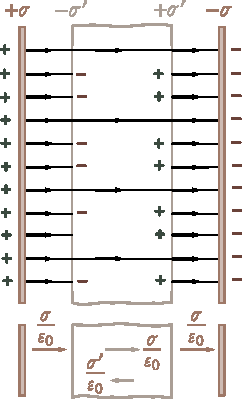
\includegraphics[scale=1]{figures/ch_02/fig_2_5.pdf}
		\caption[]{}
		\label{fig:2_5}
	\end{center}
	\vspace{-0.8cm}
\end{figure}

Cường độ trường $E_0$ bằng $\sigma/\varepsilon_0$. Cả hai trường hướng vào nhau, do đó, bên trong điện môi ta có
\begin{equation}\label{eq:2_32}
    E = E_0 - E' = E_0 - \frac{\sigma'}{\varepsilon_0} = \frac{1}{\varepsilon_0}(\sigma - \sigma').
\end{equation}

\noindent
Bên ngoài điện môi, $E=E_0$.

Độ phân cực của điện môi là do trường \eqref{eq:2_32}. Cái sau vuông góc với mặt bản. Do đó, $\ab{E}{n}=E$, và phù hợp với \eqn{2_10}, $\sigma'=\chi\varepsilon_0E$. Sử dụng giá trị này trong \eqn{2_32}, ta có
\begin{equation*}
    E = E_0 - \chi E
\end{equation*}

\noindent
từ đó
\begin{equation}\label{eq:2_33}
    E = \frac{E_0}{1 + \chi} = \frac{E_0}{\varepsilon}.
\end{equation}

\noindent
Vì vậy, trong trường hợp này, hằng số điện môi $\varepsilon$
chỉ ra điện trường bị yếu đi bao nhiêu lần trong điện môi.

Nhân \eqn{2_33} với $\varepsilon_0\varepsilon$, ta có độ điện dịch trong bản:
\begin{equation}\label{eq:2_34}
    D = \varepsilon_0 \varepsilon E = \varepsilon_0 E_0 D_0.
\end{equation}

\noindent
Do đó, độ điện dịch bên trong bản trùng với độ điện dịch của trường ngoài $D_0$. Thay $\sigma/\varepsilon_0$ cho $E_0$ trong \eqn{2_34}, ta được
\begin{equation}\label{eq:2_35}
    D = \sigma.
\end{equation}

Để tìm $\sigma'$, biểu diễn $E$ và $E_0$ trong \eqn{2_33} qua mật độ điện tích:
\begin{equation*}
    \frac{1}{\varepsilon_0} (\sigma - \sigma') = \frac{\sigma}{\varepsilon_0\varepsilon}
\end{equation*}

\noindent
từ đó
\begin{equation}\label{eq:2_36}
    \sigma' = \frac{\varepsilon - 1}{\varepsilon} \sigma.
\end{equation}

Hình \ref{fig:2_5} được vẽ với giả sử $\varepsilon=3$. Do đó, mật độ của đường sức trong điện môi bằng một phần ba bên ngoài bản. Các đường sức cách đều nhau vì trường là đồng nhất. Trong trường hợp này, $\sigma'$ có thể tìm được mà không cần dùng đến \eqn{2_36}. Đúng vậy, vì cường độ điện trường bên trong bản bằng một phần ba cường độ bên ngoài nó, nên ba đường sức bắt đầu (hoặc kết thúc) trên
điện tích ngoài, hai đường phải kết thúc (hoặc bắt đầu tương ứng) trên điện tích liên kết. Do đó mật độ điện tích liên kết phải bằng hai phần ba mật độ điện tích ngoài.

Trong hệ Gauss, cường độ điện trường $E'$ tạo ra bởi điện tích liên kết $\sigma'$ là $4\pi\sigma'$. Do đó, \eqn{2_32} trở thành
\begin{equation}\label{eq:2_37}
    E = E_0 - E' = E_0 - 4\pi\sigma'.
\end{equation}

\noindent
Mật độ điện mựt $\sigma'$ liên hệ với cường độ điện trường $E$ theo phương trình $\sigma'=\chi \ab{E}{n}$. Do đó ta có thể viết
\begin{equation*}
    E = E_0 - 4\pi\chi E
\end{equation*}

\noindent
từ đó
\begin{equation*}
    E = \frac{E_0}{1 + 4\pi\chi} = \frac{E_0}{\varepsilon}.
\end{equation*}

\noindent
Do đó, hằng số điện môi $\varepsilon$, như đối tác của nó $\varepsilon$ trong hệ SI, cho biết trường bên trong điện môi bị yếu đi bao nhiêu lần. Do đó, giá trị của $\varepsilon$ trong hệ SI và hệ Gauss là như nhau. Từ đây, tính đến Eqs. \eqref{eq:2_20} và \eqref{eq:2_28}, ta kết luận rằng độ cảm điện trong hệ Gauss ($\ab{\chi}{Gs}$) và trong hệ SI ($\ab{\chi}{SI}$) khác nhau bởi hệ số $4\pi$:
\begin{equation}\label{eq:2_38}
    \ab{\chi}{SI} = 4\pi\ab{\chi}{Gs}.
\end{equation}

\textbf{Trường bên trong một lớp cầu.} Bao bọc một quả cầu tích điện bán kính $R$ bằng một lớp cầu đồng tâm của điện môi đồng chất đẳng hướng (\fig{2_6}). Điện tích liên kết $q_1'$ phân bố với mật độ $\sigma_1'$ sẽ xuất hiện trên mặt trong của lớp ($q_1'=4\pi R_1^2\sigma_1'$), và điện tích $q_2'$ phân bố với mật độ $\sigma_2'$ sẽ xuất hiện trên mặt ngoài của nó ($q_2'=4\pi R_2^2\sigma_2'$). Dấu của điện tích $q_2'$ trùng với dấu của điện tích $q$ của quả cầu, trong khi đó $q_1'$ trái dấu.
Các điện tích $q_1'$ và $q_2'$ tạo ra một trường tại khoảng cách $r$ bên ngoài $R_1$ và $R_2$, tương ứng, nó trùng với trường của một điện tích điểm cùng độ lớn [xem \eqn{1_124}]. Điện tích $q_1'$ và $q_2'$ không tạo ra trường bên trong bề mặt mà nó được phân bố. Do đó, cường độ trường $E'$ trong điện môi là
\begin{equation*}
    E' = \frac{1}{4\pi\varepsilon_0}\frac{q_1'}{r^2} = \frac{1}{4\pi\varepsilon_0} \frac{4\pi R_1^2\sigma_1'}{r^2} = \frac{1}{\varepsilon_0} \frac{R_1^2 \sigma_1'}{r^2}
\end{equation*}

\noindent
và ngược hướng với cường độ trường $E_0$. Trường tổng hợp trong điện môi là
\begin{equation}\label{eq:2_39}
    E(r) = E_0 - E' = \frac{1}{4\pi\varepsilon_0} \frac{q}{r^2} - \frac{1}{\varepsilon_0} \frac{R_1^2 \sigma_1'}{r^2}.
\end{equation}

\begin{figure}[!htb]
	\begin{center}
		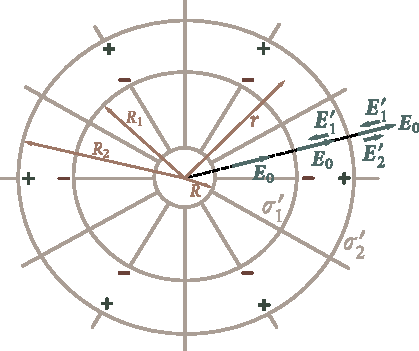
\includegraphics[scale=1.0]{figures/ch_02/fig_2_6.pdf}
		\caption[]{}
		\label{fig:2_6}
	\end{center}
	\vspace{-0.8cm}
\end{figure}

\noindent
Nó giảm tỷ lệ với $1/r^2$. Chúng ta có thể, do đó, viết
\begin{equation*}
    \frac{E(R_1)}{E(r)} = \frac{r^2}{R_1^2}\quad \Rightarrow\quad E(R_1) = E(r) \frac{r^2}{R_1^2},
\end{equation*}

\noindent
với $E(R_1)$ là cường độ điện trường trong điện môi gần với mặt trong của lớp. Chính xác là cường độ này xác định đại lượng $\sigma_1'$:
\begin{equation}\label{eq:2_40}
    \sigma_1' = \chi\varepsilon_0 E(R_1) = \chi\varepsilon_0 E(r) \frac{r^2}{R_1^2}
\end{equation}

\noindent
(tại môi điểm của bề mặt $|\ab{E}{n}|=E$).

Đưa \eqn{2_40} vào \eqn{2_39}, ta có
\begin{equation*}
    E(r) = \frac{1}{4\pi\varepsilon_0} \frac{q}{r^2} - \frac{1}{\varepsilon_0} \frac{R_1^2 \chi \varepsilon_0 E(r) r^2}{r^2 R_1^2} = E_0(r) - \chi E(r).
\end{equation*}

\noindent
Từ phương trình này, ta thấy rằng bên trong điện môi $E=E_0/\varepsilon$, và, do đó, $D=\varepsilon_0E_0$ [so sánh với phương \eqref{eq:2_33} và \eqref{eq:2_34}].

Trường bên trong điện môi thay đổi tỷ lệ với $1/r^2$. Do đó, có liên hệ $\sigma_1' :\sigma_2' = R_1 : R_2$. Từ đó,  $q_1'=q_2'$. Kết quả là, trường tạo bởi những điện tích này tại khoảng cách quá $R_2$ triệt tiêu lẫn nhau vì thế bên ngoài lớp cầu $E'=0$ và $E=E_0$.

Giả sử rằng $R_1=R$ và $R_2=\infty$, ta được trường hợp của một quả cầu tích điện chìm trong điện môi đồng nhất vô hạn và đẳng hướng. Cường độ trường bên ngoài quả cầu là
\begin{equation}\label{eq:2_41}
    E = \frac{1}{4\pi\varepsilon_0} \frac{q}{\varepsilon r^2}.
\end{equation}

\noindent
Cường độ điện trường tạo ra trong điện môi vô hạn bởi một điện tích điểm cũng tương tự.

Cả hai ví dụ xem xét trên được đặc trưng với thực tế rằng điện môi là đồng nhất và đẳng hướng, và bề mặt giới hạn nó trùng với mặt đẳng thế của điện trường của điện tích ngoài. Kết quả ta nhận được trong trường hợp này là trường hợp tổng quát. \textit{Nếu điện môi đồng nhất và đẳng hướng hoàn toàn lấp đầy thể tích giới hạn bởi bề mặt đẳng tích của trường của điện tích ngoài, thì vector điện dịch trùng với vector của cường độ điện trường của điện tích ngoài nhân với $\varepsilon_0$, và, do đó, cường độ trường bên trong điện môi là $1/\varepsilon$ của cường độ trường của điện tích ngoài}.

Nếu các điều kiện trên không được tuân thủ, vector $\vec{D}$ và $\varepsilon_0\vec{E}$ không trùng nhau. Hình \ref{fig:2_7} biểu diễn trường trong bản điện môi. Bản lệch so với mặt phẳng mang điện tích ngoài. Vector $\vec{E}'$ vuông góc với mặt bản, do đó, $\vec{E}$ và $\vec{E}_0$ là không thẳng hàng. Vector $\vec{D}$ có hướng giống $\vec{E}$, do đó, $\vec{D}$ và $\varepsilon_0\vec{E}_0$ không cùng hướng. Ta cũng có thể chỉ ra rằng chúng không cùng độ lớn.
Ở ví dụ được xem xét ở trên nhờ hình dạng được chọn đặc biệt của điện môi, trường $\vec{E}'$ chỉ khác không ở trong điện môi. Trong trường hợp tổng quát, $\vec{E}'$ có thể khác không cả ở bên ngoài điện môi. Ta đặt một thanh làm bằng điện môi vào một trường đồng chất ban đầu (\fig{2_8}). Do sự phân cực, điện tích liên kết trái dấu tạo thành ở hai đầu thanh. Trường của chúng bên ngoài thanh tương đương với trường của một lưỡng cực (các đường sức của $\vec{E}'$ là các đường nét đứt trong hình). Dễ thấy rằng trường tổng cộng $\vec{E}$ gần các đầu thanh lớn hơn trường $\vec{E}_0$.

\begin{figure}[!htb]
	\begin{minipage}[t]{0.46\linewidth}
		\begin{center}
			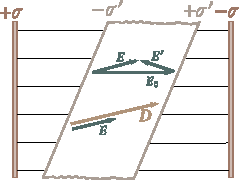
\includegraphics[scale=1.2]{figures/ch_02/fig_2_7.pdf}
			\caption[]{}
			\label{fig:2_7}
		\end{center}
	\end{minipage}
	\hfill{}%space{-0.05cm}
	\begin{minipage}[t]{0.5\linewidth}
		\begin{center}
			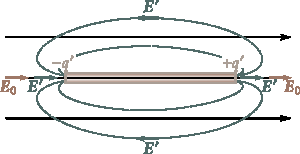
\includegraphics[scale=1.2]{figures/ch_02/fig_2_8.pdf}
			\caption[]{}
			\label{fig:2_8}
		\end{center}
	\end{minipage}
\vspace{-0.4cm}
\end{figure}

\section{Các điều kiện trên mặt phân cách hai điện môi}\label{sec:2_7}

Gần mặt phân cách giữa hai điện môi, vector $\vec{E}$ và $\vec{D}$ phải tuân theo điều kiện biên xác định từ quan hệ \eqref{eq:1_112} và \eqref{eq:2_23}:
\begin{equation*}
    \curlop{\vec{E}} = 0,\quad \divop{\vec{D}} = \rho.
\end{equation*}

Xét bề mặt phân cách giữa hai điện môi với hằng số điện môi $\varepsilon_1$ và $\varepsilon_2$ (\fig{2_9}). Chọn trục $x$ hướng bất kì trên bề mặt. Ta lấy một chu tuyến hình chữ nhật nhỏ dài $a$ và rộng $b$ mà một phần trong điện môi thứ nhất và một phần trong điện môi thứ hai. Trục $x$ đi qua trung điểm của cạnh $b$.

Giả sử rằng một trường đã được thiết lập trong điện môi thứ nhất có cường độ $\vec{E}_1$, và trong điện môi thứ hai có cường độ $\vec{E}_2$. Vì $\curlop{\vec{E}}=0$, lưu số của vector $\vec{E}$ trên chu tuyến ta đã chọn phải bằng không [xem \eqn{1_110}]. Với kích thước nhỏ của chu tuyến và hướng của chu tuyến trong \fig{2_9}, lưu số của vector $\vec{E}$ có thể được viết ở dạng
\begin{equation}\label{eq:2_42}
    \oint E_l\,\deriv{l} = E_{1,x} a - E_{2,x} a + \average{E_b} 2b
\end{equation}

\noindent
với $\average{E_b}$ là giá trị trung bình của $E_l$ trên phần vuông góc mặt phân cách của chu tuyến. Biểu thức này bằng không, ta được phương trình
\begin{equation*}
    \parenthesis{E_{1,x} - E_{2,x}} a = \average{E_b} 2b.
\end{equation*}

\noindent
Trong giới hạn, khi độ rộng $b$ của chu tuyến tiến tới không, ta có
\begin{equation}\label{eq:2_43}
    E_{1,x} = E_{2,x}.
\end{equation}

\noindent
Giá trị của hình chiếu vector $\vec{E}_1$ và $\vec{E}_2$ lên trục $x$ được lấy ở lân cận mặt phân cách giữa ranh giới của các điện môi.

Phương trình \eqref{eq:2_43} được tuân thủ khi trục $x$ được chọn tùy ý. Chỉ có một điều quan trọng là trục này ở trong mặt phẳng phân cách giữa các điện môi. Nghiên cứu \eqn{2_43} chỉ ra rằng với trục $x$ được chọn như thế thì $E_{1,x}=0$, hình chiếu của $E_{2,x}=0$ cũng sẽ bằng không. Điều này có nghĩa là vector $\vec{E}_1$ và $\vec{E}_2$ tại hai điểm gần nhau được lấy ở hai phía đối diện của mặt phân cách là nằm trong cùng mặt phẳng với pháp tuyến của mặt phân cách. Biểu diễn mỗi vector $\vec{E}_1$ và $\vec{E}_2$ ở dạng tổng các thành phần pháp tuyến và tiếp tuyến:
\begin{equation*}
    \vec{E}_1 = \vec{E}_{1,n} + \vec{E}_{1,\tau},\quad \vec{E}_2 = \vec{E}_{2,n} + \vec{E}_{2,\tau}.
\end{equation*}

\noindent
Phù hợp với \eqn{2_43}
\begin{equation}\label{eq:2_44}
    E_{1,\tau} = E_{2,\tau}.
\end{equation}

\noindent
Ở đây $\vec{E}_{i,\tau}$ là hình chiếu của vector $\vec{E}_i$ lên vector đơn vị $\hatvec{\tau}$ hướng dọc theo giao tuyến của mặt phân cách điện môi với mặt phẳng chứa vector $\vec{E}_1$ và $\vec{E}_2$.

\begin{figure}[!htb]
	\begin{minipage}[t]{0.48\linewidth}
		\begin{center}
			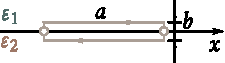
\includegraphics[scale=1.0]{figures/ch_02/fig_2_9.pdf}
			\caption[]{}
			\label{fig:2_9}
		\end{center}
	\end{minipage}
	\hfill{}%space{-0.05cm}
	\begin{minipage}[t]{0.48\linewidth}
		\begin{center}
			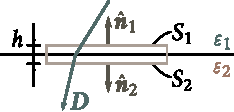
\includegraphics[scale=1.0]{figures/ch_02/fig_2_10.pdf}
			\caption[]{}
			\label{fig:2_10}
		\end{center}
	\end{minipage}
\vspace{-0.4cm}
\end{figure}

Thay thế phù hợp với \eqn{2_21} Hình chiếu của vector $\vec{D}$ chia $\varepsilon_0\varepsilon$ cho hình chiếu của vector $\vec{E}$, ta có tỷ lệ
\begin{equation*}
    \frac{D_{1,\tau}}{\varepsilon_0\varepsilon_1} = \frac{D_{2,\tau}}{\varepsilon_0\varepsilon_2}
\end{equation*}

\noindent
do đó
\begin{equation}\label{eq:2_45}
    \frac{D_{1,\tau}}{D_{2,\tau}} = \frac{\varepsilon_1}{\varepsilon_2}.
\end{equation}

Bây giờ ta lấy một mặt trụ ảo chiều cao $h$ trên mặt phân cách giữa giữa các điện môi (\fig{2_10}). Đáy $S_1$ nằm trong điện môi thứ nhất, và đáy $S_2$ trong cái thứ hai. Hai đáy có kích thước giống nhau ($S_1=S_2=S$) và nhỏ tới mức mà trong giới hạn của chúng, trường có thể xem là đồng nhất. Áp dụng định lý Gauss [xem \eqn{2_25}] vào mặt này. Nếu không có điện tích ngoài trên mặt phân cách giữa các điện môi, vế phải trong \eqn{2_25} bằng không. Do đó, $\Phi_D=0$.

Thông lượng qua mặt $S_1$ là $D_{1,n}S$, với $D_{1,n}$ là hình chiếu của vector $\vec{D}$ trong điện môi thứ nhất lên pháp tuyến $\hatvec{n}_1$. Tương tự, thông lượng qua đáy $S_2$ là $D_{2,n}S$, với $D_{2,n}$ là hình chiếu của vector $\vec{D}$ trong điện môi thứ hai lên pháp tuyến $\hatvec{n}_2$. Thông lượng qua
mặt bên có thể được viết ở dạng $\average{D}_n\ab{S}{side}$, với $\average{D}_n$ là giá trị của $D_n$ trung bình trên toàn bộ mặt bên, và $\ab{S}{side}$ là độ lớn của mặt này. Do đó có thể viết
\begin{equation}\label{eq:2_46}
    \Phi_D = D_{1,n} S + D_{2,n} S + \average{D}_n\ab{S}{side} = 0.
\end{equation}

\noindent
Nếu độ cao $h$ của hình trụ tiến tới không, thì $\ab{S}{side}$ cũng tiến tới không. Do đó, trong giới hạn, ta có
\begin{equation*}
    D_{1,n} = - D_{2,n}.
\end{equation*}

\noindent
Ở đây $D_{i,n}$ là hình chiếu lên $\hatvec{n}_i$ của vector $\vec{D}$ trong điện môi thứ $i$ ở rất gần mặt phân cách của nó với điện môi khác. Dấu của hình chiếu khác nhau vì pháp tuyến $\hatvec{n}_1$ và $\hatvec{n}_2$ của đáy hình trụ ngược hướng. Nếu ta chiếu $\vec{D}_1$ và $\vec{D}_2$ lên cùng pháp tuyến, ta có điều kiện
\begin{equation}\label{eq:2_47}
    D_{1,n} = D_{2,n}.
\end{equation}

Sử dụng \eqn{2_21} để thay thế hình chiếu của $\vec{D}$ với hình chiếu tương ứng của vector $\vec{E}$ nhân bởi $\varepsilon_0\varepsilon$, ta có liên hệ
\begin{equation*}
    \varepsilon_0 \varepsilon_1 E_{1,n} = \varepsilon_0 \varepsilon_2 E_{2,n}
\end{equation*}

\noindent
do đó
\begin{equation}\label{eq:2_48}
    \frac{E_{1,n}}{E_{2,n}} = \frac{\varepsilon_2}{\varepsilon_1}.
\end{equation}

Kết quả ta nhận được chỉ ra rằng khi đi qua mặt phân cách giữa hai điện môi, thành phần pháp tuyến của vector $\vec{D}$ và thành phần pháp tuyến của vector $\vec{E}$ thay đổi liên tục. Tuy nhiên, thành phần tiếp tuyến của vector $\vec{D}$ và thành phần
pháp tuyến của vector $\vec{E}$, bị gián đoạn khi đi qua mặt phân cách.

Phương trình \eqref{eq:2_44}, \eqref{eq:2_45}, \eqref{eq:2_47}, và \eqref{eq:2_48} xác định các điều kiện mà vector $\vec{E}$ và $\vec{D}$ phải tuân theo trên mặt phân cách giữa hai điện môi (nếu không có điện tích ngoài trên mặt phân cách này). Ta đã nhận được những phương trình này cho một trường tĩnh điện. Chúng cũng đúng cho trường thay đổi theo thời gian (xem
\sect{16_3}).

Các điều kiện ta đã tìm được vẫn đúng cho mặt phân cách giữa điện môi và chân không. Trong trường hợp này, một trong các hằng số điện môi phải bằng một đơn vị.

Ta phải chú ý rằng điều kiện \eqref{eq:2_47} có thể nhận được trên cơ sở của sự thật rằng các đường điện dịch đi qua mặt phân cách giữa hai điện môi mà không bị gián đoạn (\fig{2_11}). Theo
các nguyên tắc để vẽ những đường này, số đường sức tới diện tích $\Delta{S}$ từ điện môi thứ nhất là $D_1\Delta{S}_1=D_1\Delta{S}\cos\alpha_1$. Tương tự, số đường sức đi ra từ diện tích $\Delta{S}$ vào điện môi thứ hai là $D_2\Delta{S}_2=D_2\Delta{S}\cos\alpha_2$. Nếu các đường sức không bị gián đoạn tại mặt phân cách, cả hai số này phải bằng nhau:
\begin{equation*}
    D_1\Delta{S}\cos\alpha_1 = D_2\Delta{S}\cos\alpha_2.
\end{equation*}

\noindent
Rút gọn $\Delta{S}$ và tính đến tích $D\cos\alpha$ cho giá trị của thành phần pháp tuyến vector $\vec{D}$, ta nhận được điều kiện \eqref{eq:2_47}.

Các đường điện dịch bị cong (khúc xạ) trên mặt phân cách giữa các điện môi, do góc $\alpha$ giữa pháp tuyến với mặt phân cách và đường $\vec{D}$ thay đổi. \fig{2_12} chỉ ra rằng
\begin{equation*}
    \tan\alpha_1 : \tan\alpha_2 = \frac{D_{1,\tau}}{D_{1,n}} : \frac{D_{2,\tau}}{D_{2,n}}
\end{equation*}

\noindent
Từ các phương trình \eqref{eq:2_45} và \eqref{eq:2_47}, ta có định luật của sự khúc xạ điện dịch:
\begin{equation}\label{eq:2_49}
    \frac{\tan\alpha_1}{\tan\alpha_2} = \frac{\varepsilon_1}{\varepsilon_2}.
\end{equation}

\noindent
Khi các đường điện dịch đi vào một điện môi với hằng số điện môi $\varepsilon$ bé hơn, góc tạo bởi chúng với pháp tuyến giảm, do đó, các đường cách xa nhau; trái lại, khi các đường đi vào một điện môi với hằng số điện môi $\varepsilon$ lớn hơn, chúng trở nên gần nhau hơn.

\begin{figure}[!htb]
	\begin{minipage}[t]{0.48\linewidth}
		\begin{center}
			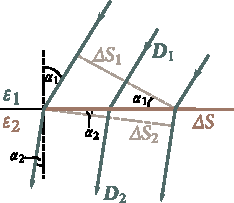
\includegraphics[scale=1.1]{figures/ch_02/fig_2_11.pdf}
			\caption[]{}
			\label{fig:2_11}
		\end{center}
	\end{minipage}
	\hfill{}%space{-0.05cm}
	\begin{minipage}[t]{0.48\linewidth}
		\begin{center}
			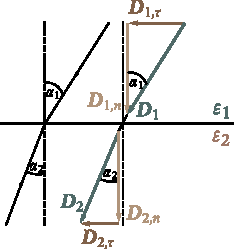
\includegraphics[scale=1.1]{figures/ch_02/fig_2_12.pdf}
			\caption[]{}
			\label{fig:2_12}
		\end{center}
	\end{minipage}
\vspace{-0.4cm}
\end{figure}

\section{Lực tác dụng lên một điện tích trong điện môi}\label{sec:2_8}

Nếu ta đưa vào điện trường trong chân không một vật mang điện có kích thước nhỏ tới nỗi mà trường ngoài trong vật thể có thể được coi là đồng nhất, thì vật thể sẽ chịu lực
\begin{equation}\label{eq:2_50}
    \vec{F} = q \vec{E}.
\end{equation}

\noindent
Để đặt một vật mang điện trong trường được tạo ra trong một điện môi, phải có một cái hốc trong điện môi. Trong một điện môi lỏng, vật mang điện tự nó tạo hốc bằng cách dịch chuyển điện môi khỏi thể tích nó chiếm. Trường bên trong hốc $\ab{\vec{E}}{cav}$ sẽ khác với với trường trong một điện môi liên tục. Do đó, ta không thể tính lực tác dụng lên vật mang điện đặt trong hốc như là tích của điện tích $q$ và cường độ trường $\vec{E}$ trong điện môi trước khi vật thể được đưa vào nó.

Khi tính lực tác dụng lên một vật mang điện trong điện môi lỏng, ta phải tính đến các trường hợp khác. Sức căng cơ học được thiết lập trên ranh giới với vật thể trong điện môi. Nó tạo ra một lực cơ học phụ $\ab{\vec{F}}{ten}$ tác dụng lên vật thể.

Do đó, lực tác dụng lên một vật mang điện trong điện môi, nói chung, không thể được xác định bởi \eqn{2_50}, và nó thường rất khó để tính toán. Những tính toán này cho một kết quả rất thú vị đối với một điện môi lỏng. Kết quả của lực điện $q\ab{\vec{E}}{cav}$ và lực cơ học $\ab{\vec{F}}{ten}$ được tìm thấy bằng chính xác với $q\vec{E}$, với $\vec{E}$ là cường độ trường trong điện môi liên tục
\begin{equation}\label{eq:2_51}
    \vec{F} = q\ab{\vec{E}}{cav} + \ab{\vec{F}}{ten} = q\vec{E}.
\end{equation}

Cường độ trường trong điện môi đồng chất vô hạn tạo ra bởi một điện tích được xác định bởi \eqn{2_49}. Do đó, ta có biểu thức sau cho lực tương tác giữa hai điện tích điểm chìm trong điện môi đồng chất vô hạn:
\begin{equation}\label{eq:2_52}
    F = \frac{1}{4\pi\varepsilon_0} \frac{q_1q_2}{\varepsilon r^2}.
\end{equation}

\noindent
Công thức này thể hiện định luật Coulomb cho điện tích trong điện môi. Nó chỉ đúng cho điện môi điện môi lỏng.

Một vài tác giả đặc trưng \eqn{2_52} như ``biểu thức tổng quát nhất của định luật coulomb''. Trong vấn đề này, ta sẽ đề cập đến Richard P. Feynman: ``Nhiều cuốn sách cũ hơn về điện bắt đầu với định luật 'quan trọng' mà lực giữa hai điện tích là\ldots [\eqn{2_52} được cho]\ldots, Một quan điểm mà hoàn toàn không thỏa đáng. Đầu tiên, nó không đúng về mặt tổng quát; nó chỉ đúng cho môi trường lấp đầy bởi chất lỏng. Thứ hai, nó phụ thuộc vào sự thật rằng $\varepsilon$ là một hằng số chỉ xấp xỉ đúng cho hầu hết vật liệu thực tế''\footnote{R. P. Feynman, R. B. Leighton, M. Sands. The Feynman Lectures on Physics. Vol. II. Reading, Mass., Addison-Wesley (1965), p. 10-8.}.

Ta sẽ không trả lời câu hỏi liên quan đến lực tác dụng lên một điện tích nằm trong một cái hốc làm từ điện môi rắn.

\section{Sắt điện}\label{sec:2_9}

Có một nhóm vật liệu có thể có tính chất phân cực tự phát khi không có trường ngoài. Chúng được gọi là \textbf{sắt điện}. Hiện tượng này lần đầu tiên được phát hiện ở muối Rochelle, và nghiên cứu cụ thể đầu tiên về tính chất điện của muối này được thực hiện bởi nhà vật lý người Liên Xô I. Kurchatov và P. Kobeko.

Chất sắt điện khác các điện môi ở một số đặc điểm :

1. Trong khi hằng số điện môi $\varepsilon$ của điện môi bình thường chỉ vài đơn vị, một số ngoại lệ lớn (ví dụ, nước có $\varepsilon=81$), hằng số điện môi của chất sắt điện có thể có bậc cỡ vài nghìn.

2. Sự phụ thuộc của $P$ vào $E$ là không tuyến tính (xem nhánh $1$ của đường cong trong \fig{2_13}). Do đó, hằng số điện môi phụ thuộc vào cường độ trường.

3. Khi trường thay đổi, giá trị của độ phân cực $P$ (và, do đó, của điện dịch $D$) trễ pha so với cường độ trường $E$. Kết quả là, $P$ và $D$ được xác định không chỉ bởi giá trị của $E$ tại thời điểm đó, mà còn vào giá trị trước đó của $E$, tức là, chúng phụ thuộc vào trạng thái trước đó của điện môi. Hiện tượng này gọi là \textbf{điện trễ} (từ tiếng Hy Lạp ``husterein''---nghĩa là tới trễ). Khi trường thay đổi tuần hoàn, sự phụ thuộc của $P$ vào $E$  tuân theo đường cong trong \fig{2_13} và được gọi là  \textbf{lặp điện trễ}.
Khi trường bắt đầu xuất hiện, độ phân cực tăng với $E$ theo nhánh $1$ của đường cong. $P$ giảm dọc theo nhánh $2$. Khi $E$ biến mất, vật liệu giữ lại một giá trị của độ phân cực $\ab{P}{r}$ gọi là \textbf{độ phân cực dư}. Độ phân cực chỉ biến mất dưới tác động của một trường hướng ngược lại $\ab{E}{c}$. Giá trị này của cường độ trường gọi là \textbf{lực cưỡng bức}. Khi $E$ thay đổi hơn nữa, ta nhận được nhánh $3$ của vòng lặp điện trễ, vân vân.

\begin{figure}[!htb]
    \begin{center}
		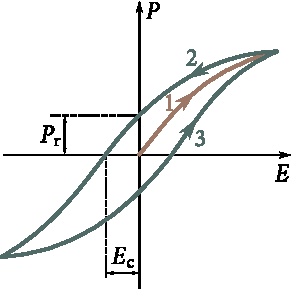
\includegraphics[scale=1.0]{figures/ch_02/fig_2_13.pdf}
		\caption[]{}
		\label{fig:2_13}
	\end{center}
    \vspace{-0.8cm}
\end{figure}

Hành vi của sự phân cực của chất sắt điện là tương tự với sự từ hóa của chất sắt từ (xem \sect{7_9}), và đó là nguồn gốc cái tên của nó.

Chỉ có chất kết tinh không có tâm đối xứng mới có thể là chất sắt điện. Ví dụ, tinh thể của muối Rochelle thuộc hệ hình thoi (xem Sec. 13.2 of Vol. I). Tương tác của các hạt trong tinh thể sắt điện dẫn đến sự thật rằng moment lưỡng cực của chúng xếp song song tự phát với cái khác. Trong các trường hợp riêng biệt, hướng giống nhau của moment lưỡng cực mở rộng ra toàn bộ tinh thể. Tuy nhiên, thông thường, các vùng xuất hiện trong tinh thể mà trong đó moment lưỡng cực là song song với nhau, nhưng các hướng của sự phân cực trong các vùng khác nhau là khác nhau. Do đó, moment tổng cộng của toàn bộ tinh thể có thể bằng không. Vùng có sự phân cực tự phát còn được gọi là \textbf{miền}. Dưới tác dụng của trường ngoài, moment của vùng xoay như một tổng thể duy nhất, sắp xếp chúng theo hướng của trường.

Mỗi chất sắt điện có một nhiệt độ mà tại đó vật chất mất đặc tính khác biệt của nó và trở thành điện môi bình thường. Nhiệt độ này được gọi là \textbf{điểm Curie }. Muối Rochelle có hai điểm Curie, cụ thể là, \SI{-15}{\degreeCelsius} và \SI{+22}{\degreeCelsius}, và nó chỉ biểu hiện như chất sắt điện giữa hai nhiệt độ này. Đặc tính điện của nó trở nên bình thường tại nhiệt độ dưới \SI{-15}{\degreeCelsius} và trên \SI{+22}{\degreeCelsius}.
